\documentclass[../main.tex]{subfiles}
\graphicspath{{\subfix{../IMAGES/}}}

\begin{document}
\localtableofcontents

\subsection{Introduction}

Le système mécanique est un ensemble d'éléments intégrés de manière à recevoir, transformer et restituer de l'énergie, de la matière et de l'information pour accomplir une fonction spécifique.\\

Un système mécanique peut être décomposée en plusieurs couches de sous-systèmes et éléments. A chaque sous-système on peut associer une fonction spécifique.\\

Cinématique ou dynamique ? \begin{itemize}
    \item Cinématique : mouvement de corps rigides\\
    \item Dynamique : tient compte de la déformation des éléments\\
\end{itemize}

\quad \underline{Cinématique : définition}\\
La cinématique étudie le mouvement, la vitesse et l'accélération de points et de corps rigides dans l'espace.\\

Une chaîne cinématique est un ensemble de corps rigides liés entre eux.\\

Soit un mécanisme avec $N_p$ éléments (bar etc.. et ne compter le bâti qu'une fois), $N_L$ liaisons.\\

\begin{itemize}
    \item Degré de mobilité d'une chaîne cinématique : détermine le nombre de paramètres indépendants nécessaires pour fixer tout élément dans l'espace\\
    \item Déterminer le degré de mobilité : \begin{itemize}
        \item nombre degrés de liberté par rapport à un élément de base : $6(N_p-1)$\\
        \item degré de liaison du couple i : $n_{si} = 6-n_{ci}$ (avec $n_{ci}$ le degré de liberté de la liaison)\\
        \item les liaisons enlèvent des degrés de libertés : $\sum_{i=1}^{N_L} n_{si}= \sum_{i=1}^{N_L}6-n_{ci} = 6N_L - \sum_{i=1}^{N_L} n_{ci}$\\
        \item degré de mobilité : $m_c = 6(N_p-1)-\sum_{i=1}^{N_L} n_{si} = 6(N_p-N_L-1) + \sum_{i=1}^{N_L} n_{ci}$\\
    \end{itemize}
\end{itemize}

Degré de liaison et de liberté d'une liaison : \begin{table}[hbt!]
    \centering
    \begin{tabular}{|c|c|c|}
    \hline
        Fonctions & Degré de liaison & Degré de liberté \\
        \hline
         1 : Ponctuelle & 1 & 5\\
         2 : Linéaire angulaire & 2 & 4\\
         3 : Linéaire rectiligne & 2 & 4\\
         4 : rotule & 3 & 3\\
         5 : surfacique (2D) & 1 & 2\\
         \hline
    \end{tabular}
\end{table}

Pour un système plan, on a : \begin{equation}
    m_c = 3(N_p-1)-2N_{L1} -N_{L2}
\end{equation}

Avec : \begin{itemize}
    \item $N_{L1}$ : nombre de liaisons avec un degré de liaison = 2 (liberté = 1)\\
    \item $N_{L2}$ : nombre de liaisons avec un degré de liaison = 1 (liberté = 2)\\
\end{itemize}
Les équations de liaison limitent les coordonnées indépendantes. La différence entre le nombre de coordonnées et les équations de liaison détermine le nombre de coordonnées indépendantes et donc le nombre de degré de mobilité.\\

\subsection{Loi de mouvement cinématique}
Soit : \begin{itemize}
    \item $q_p$ la coordonnée généralisée de l'élément p\\
    \item $Q_p$ l'effort généralisé appliqué à l'élément p\\
\end{itemize}

\quad \underline{Loi d'espace :}\\
Elle décrit intégralement le mouvement d'une pièce. On exprime tout le mouvement selon une coordonnée généralisée (souvent celle du meneur) $x_i = x_i(q)$.\\

On a dès lors la vitesse : $\dot{x}_i = x'_i(q)\dot{q}(t)$\\
Ainsi que l'accélération : $\Ddot{x}_i = x"_i(q) \dot{q}^2(t) + x'_i(q) \Ddot{q}(t)$\\

\begin{itemize}
    \item Rapport de transmission : $i=\frac{\omega_{\text{entrée}}}{\omega_{\text{sortie}}} = -\frac{Z_{\text{sortie}}}{Z_{\text{entrée}}}$\\
    \item Système uniforme/homocinétique/synchrone si i=cst ou $I_{reduit} = cst$\\
    \item Système non-uniforme/hétérocinétique si i$\neq$cst\\
\end{itemize}

On trouve ensuite les lois de mouvements à l'aide des équations de Lagrange : $L = T-U$\\
$\frac{d}{dt}(\frac{\partial L}{\partial \dot{q}_n}) - (\frac{\partial L}{\partial q_n}) = Q_n^*$\\

On a alors pour l'énergie cinétique : \begin{equation}
    \begin{gathered}
        T = \frac{1}{2}\sum_i [m_i(\dot{x}^2_i + \dot{y}^2_i) + J_i \dot{\varphi}^2_i]\\
        T = \frac{1}{2} \dot{q}^2 \sum_i [m_i (x_i'^2+y_i'^2) + J_i \varphi_i'^2]\\
        T = \frac{1}{2} I(q) \dot{q}^2\\
    \end{gathered}
\end{equation}

Où $I(q)$ est l'inertie globale du système mécanique.\\

Réduction des efforts extérieurs à la coordonnée générale menante $q$ : \\
\begin{equation}
    Q^* = \sum_i (F_{xi} \frac{\partial x_i}{\partial q} + F_{yi} \frac{\partial y_i}{\partial q} + M_i \frac{\partial \varphi_i}{\partial q}) = Q_m^* - Q_e^*
\end{equation}

Avec $Q_m^*$ les efforts moteur et $Q_e^*$ les efforts résistants.\\

\quad \underline{Système à 1 degré de mobilité :}\\
On obtient par Lagrange : $I(q) \Ddot{q} + \frac{1}{2} I'(q) \dot{q}^2 + U'(q) = Q_m^* - Q_e^*$\\

\subsubsection{Discrétisation des masses}
On remplace la masse et l'inertie au centre de gravité par des masses équivalentes aux endroits où les lois sont plus simples.\\

Principe d'équivalence : \begin{equation}
    \begin{gathered}
        m =  m_A + m_B\\
        m_Aa = m_Bb\\
        J_G = m_A a^2 + m_B b^2\\
    \end{gathered}
\end{equation}

\subsubsection{Efforts d'inertie}
Dans un repère, on a par la loi de Newton : \begin{equation}
    \Vec{F} = m\Vec{a}_a(A) + m\Vec{\Omega} \Vec{AP} + m\Vec{\Omega} \times (\Vec{\Omega} \times \Vec{AP}) + m\Vec{a}_r(P) + 2m\Vec{\Omega}\times \Vec{v}_r
\end{equation}

Pour un corps solide ($\Vec{a}_r(P) = 0$, $\Vec{v}_r = 0$) On a : $0 = \Vec{F}-[m\Vec{a}_a(A) + m\dot{\Vec{\Omega}} \Vec{AP} + m\Vec{\Omega} \times (\Vec{\Omega} \times \Vec{AP})]$ (principe d'alembert)\\

Les deux efforts (utile et inertie) limitent la vitesse du système. L'effort d'inertie est un effort mesuré dans le repère A.\\

Ainsi : \begin{itemize}
    \item $0 = \Vec{F} + \Vec{F}_{inertie} \Rightarrow \Vec{F}_{inertie} = -ma_a$\\
    \item $0 = \Vec{M} + \Vec{M}_{inertie} \Rightarrow \Vec{M}_{inertie} = -J_G \alpha_a$\\
\end{itemize}

De manière générale : $F_{inertie} = -m_G [x"_G(q) \dot{q}^2(t) + x'_G(q) \Ddot{q}(t)]$\\

\begin{itemize}
    \item Lorsque la vitesse est constante ($\dot{q} = cst$) et que le système est non-uniforme, les efforts sont proportionnels au carré de la vitesse\\
    \item Lorsque le système est uniforme ($I(q) = cst$) les efforts sont proportionnels à l'accélération du système.\\
\end{itemize}

\subsection{Limitations par les efforts d'inertie}

Les éléments sont chargés par : \begin{itemize}
    \item une précontrainte : $\sigma_0$\\
    \item une contrainte d'inertie : $\sigma_I = C_I \rho v^2$\\
    \item une contrainte utile : $\sigma_U= C_U F$\\
\end{itemize}

Sous l'hypothèse des contraintes parallèles, on a un critère de dimensionnement : $\sigma_0 + C_I \rho v^2 + C_U F_U \leq \frac{\sigma_{lim}}{S}$, S le coefficient de sécurité.\\

L'effort et la puissance utile deviennent : \begin{itemize}
    \item $F_U \leq \frac{1}{C_U} [\frac{\sigma_{lim}}{S} -  \sigma_0 - C_I \rho v^2]$\\
    \item $P_U = F_{U max} v = \frac{1}{C_U} [\frac{\sigma_{lim}}{S} - \sigma_0 - C_I \rho v^2] v$\\
\end{itemize}

En dérivant les équations, on trouve donc les valeurs optimales : \begin{itemize}
    \item $v_{opt} = \sqrt{\frac{1}{3}} v_{max}$\\
    \item $F_{U opt} = \frac{2}{3} F_{U max}$\\
    \item $P_{max} = \frac{2}{3\sqrt{3}} F_{U max} v_{max}$\\
\end{itemize}

\subsection{Équilibrage des efforts d'inertie}
La résultante des n éléments est appliquée au centre de gravité G du mécanisme : $\Vec{F}_I = -\sum_k m_k \Vec{a}_k = m\Vec{a}_G$\\

Les efforts d'inertie d'une chaîne cinématique plane à 1 degré de mobilité sont donc : \begin{itemize}
    \item $F_{Ix} = -\sum_k m_k [x_{Gk}"(q) \dot{q}^2(t) + x_{Gk}'(q) \Ddot{q}(t)]$\\
    \item $F_{Iy} = -\sum_k m_k [y_{Gk}"(q) \dot{q}^2(t) + y_{Gk}'(q) \Ddot{q}(t)]$\\
\end{itemize}

Le couple d'inertie appliqué au bâti est donc : $M_{IG} = -\sum_k J_{Gk} [\varphi_{Gk}"(q) \dot{q}^2(t) + \varphi_{Gk}'(q) \Ddot{q}(t)]$\\

Auquel on peut rajouter le moment des forces d'inertie par rapport au point O : $M_{I0} = M_{IG} + \sum_k \Vec{r}_{Gk} \times \Vec{F}_{Ik}$\\

L'équilibrage parfait est atteint lorsque $\Vec{F}_I = 0$, $M_{I0} = 0$\\

\subsection{Mouvement de groupe}
\warning Il est important de noter que les équations sont globales ! Il faut remettre selon le bon référentiel : \begin{equation}
    \begin{gathered}
        M_m^* = i M_m\\
        M_e^* = \frac{1}{i} M_e\\
        J_m^* = i^2 J_m\\
        J_e^* = \frac{1}{i^2} J_e\\
    \end{gathered}
\end{equation}


Soit l'effort cinétique pour un groupe rotatif : $Q_m^* - Q_e^* = I(q) \Ddot{q} + \frac{1}{2} I'(q) \dot{q}^2 + U'(q)$
Soit : $M_{ec} = J_e(\varphi) \dot{w} + \frac{1}{2} \frac{d J_e (\varphi)}{d\varphi} \omega^2 + \frac{d U_e (\varphi)}{d\varphi} + M_e^*$\\

Ou encore $M_{mc} = M_m^* - \frac{dU_m (\varphi)}{d\varphi} - \frac{1}{2} \frac{d J_m (\varphi)}{d\varphi} \omega^2 - J_m (\varphi) \dot{\omega}$\\

$M_{mc}$ : le moment du moteur cinématique et $M_{ec}$ : le moment d'entraînement cinématique\\

On a également : \begin{equation}
    M_m^* - M_e^* = (J_m^* + J_e^*) \dot{\omega} + \frac{1}{2} (J_m^{*'} + J_e^{*'})\omega^2 + (U_m' + U_e')
\end{equation}

Le groupe : 
\begin{itemize}
    \item accélère si $M_m^* > M_e^*$\\
    \item ralentit si $M_m^* < M_e^*$\\
    \item la vitesse en régime stationnaire (point de fonctionnement) $M_m^*(\omega_0) = M_e^*(\omega_0)$\\
\end{itemize}

On a également une \textbf{condition de stabilité} : \begin{equation}
    \frac{d M_m^*}{d\omega} < \frac{d M_e^*}{d\omega}
\end{equation}

\subsubsection{Irrégularité de marche}
Soit une variation d'allure voire des efforts cycliques. On a $\overline{\omega} = \frac{1}{T} \int_t^{t+T} \omega(t) dt$\\

Les fluctuations sont exprimées par le \textbf{facteur d'irrégularité} : \begin{equation}
    \delta = \frac{\omega_{max}-\omega_{min}}{\overline{\omega}}
\end{equation}

Pour des fluctuations périodiques avec des écarts faibles, on a $\overline{\omega} = \frac{1}{2}(\omega_{max} + \omega_{min})$, $\delta = 2 \frac{\omega_{max} - \omega_{min}}{\omega_{max} + \omega_{min}}$\\

On peut exprimer l'accélération d'un groupe comme : ($M_B$ est le moment créé par l'ajout d'un mécanisme supplémentaire) : \begin{equation}
    \dot{\omega} = \frac{1}{J_m + J_e} [(M_m^* - M_e^*) - (U_m' + U_e') - \frac{1}{2} (J_m' + J_e')\omega^2 + M_B]
\end{equation}

\subsubsection{Démarrage}
Consiste à fournir de l'énergie au groupe pour décoller la machine et augmenter l'énergie cinétique des éléments en mouvement.\\
L'étude de démarrage permet de déterminer le temps de démarrage, l'espace parcouru pendant la phase de démarrage ainsi que l'évolution de la vitesse.\\

On doit avoir $M_{md0} > M_{ed0}$. Si ce n'est pas possible, il faut utiliser un embrayage.\\

Pour un système uniforme, on a : \begin{equation}
    \frac{dt}{J_m^* + J_e^*} = \frac{d \omega}{M_m^* - M_e^*}
\end{equation}

Cela permet donc de trouver le temps de démarrage.\\

\subsubsection{Freinage}
Il existe trois moyens : \begin{itemize}
    \item $Q(t) = Q_0$, frottement\\
    \item $Q(t) = Q_0 \frac{\dot{q}}{\dot{q}_0}$, frein de Foucault\\
    \item $Q(t) = Q_0 (\frac{\dot{q}}{\dot{q}_0})^2$, aérodynamique\\
\end{itemize}

Le frein par frottement est le plus efficace pour arrêter une machine. Le frein fonction de la vitesse n'arrête pas le système.\\

Pour un frein par frottement, on a une énergie dissipée équivalente à : \begin{equation}
    W_f = \int_0^{\varphi_a} M d\varphi + \frac{1}{2} (J_f + J) \omega_0^2
\end{equation}

\subsection{Modélisation}

Il existe trois types de modèles en conception mécanique : \begin{itemize}
    \item Statique : efforts d'inertie sont négligeables par rapport aux efforts statiques (machines très lentes)\\
    \item Cinématique : éléments sont supposés indéformables, tient compte des efforts d'inertie provoqués par les grands mouvements\\
    \item Dynamique : éléments sont déformables, tient compte des efforts d'inertie provoqués pas les grands mouvements et par les mouvements de vibration\\
\end{itemize}

Le modèle dynamique d'un oscillateur élémentaire est : $\frac{1}{\omega_0^2} \Ddot{Q}_{R-D} + \frac{2\eta}{\omega_0} \dot{Q}_{R-D} + Q_{R-D} = Q \cos(\Omega t)$, $\omega_0 = \sqrt{k/I}$, $\eta = \frac{c}{2I\omega_0}$, avec $Q_{R-D} $ l'effort transmis par le ressort.\\

En régime permanent, on a $Q_{R-D} = Q \mu_1 \cos(\Omega t - \varphi_1)$, $\varphi_1 = \arctan(\frac{4\eta \beta}{1-\beta^2})$, $\beta = \frac{\Omega}{\omega_0}$, $\mu_1 = \frac{1}{\sqrt{(1-\beta^2)^2 + 4 \eta^2 \beta^2}}$\\

Avec le modèle cinématique, on obtient $Q_{R-C} = Q\cos(\Omega t)$.\\

L'erreur relative est donc de $e = \frac{\mu_1-1}{\mu_1}$.\\

En fixant l'erreur limite, on peut trouver la valeur limite de $\mu_1$ : $\mu_{1Lim} = \frac{1}{1-\lvert e_{lim}\rvert}$\\

Le modèle cinématique ne tient pas compte de la nature vibratoire mais fournit un résultat acceptable lorsque $\Omega \leq \Omega_0 \sqrt{e_{lim}}\lvert_{\eta=0}$\\

L'amortissement influence peu le $\beta_{lim}$. Le modèle cinématique s'écarte fortement lorsque la pulsation relative s'approche de la pulsation propre. Pour une excitation $\Omega \leq 0.22\omega_0$ (erreur de 5$\%$) on peut se contenter d'un modèle cinématique.\\

Comme $\omega_1 = \omega_0 \sqrt{1-\eta^2}$, il est raisonnable de négliger l'amortissement pour une estimation de la pulsation propre. En négligeant l'amortissement, on commet une erreur par excès ainsi qu'une erreur de phase substantielle. Pour une erreur admissible, il existe deux plages où l'on peut négliger l'amortissement.\\

\subsection{Discrétisation dynamique}

\begin{figure}[hbt!]
    \centering
    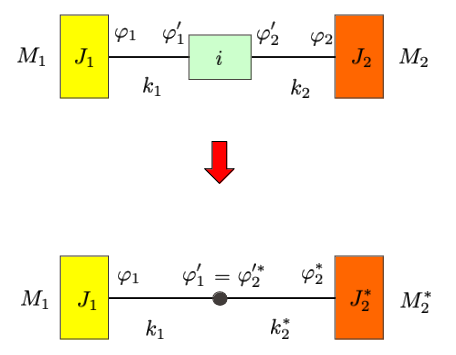
\includegraphics[width=.6\textwidth]{IMAGES/constru/dsm1.png}
\end{figure}

Réduction à la coordonnée d'entrée 1 : $i = \frac{\dot{\varphi}_1}{\dot{\varphi}_2}$\\
\begin{itemize}
    \item $M_2^* = M_2 \frac{1}{i}$\\
    \item $J_2^* = J_2 \frac{1}{i^2}$\\
    \item $m_2^* = m_2 \frac{1}{i^2}$\\
    \item $k_2^* = k_2 \frac{1}{i^2}$\\
\end{itemize}

\warning Approche seulement valide pour des déformations faibles ! Si plusieurs i dans le système, prendre tous ceux présent avant la position.\\

En combinant les équations pour les deux masses, on a $\Ddot{\psi} + k_{eq} \frac{I_1 + I_2}{I_1I_2} \psi = \frac{M_1}{I_1}$ ($M_2= 0$)\\

De manière générale, on modélise un système de manière à ce qu'on ait deux fréquences propres au-delà du spectre d'excitation. \\
\begin{itemize}
    \item Si les pulsations propres sont loin du domaine d'excitation, le calcul cinématique est suffisant\\
    \item Si les pulsations propres sont en partie sur le domaine d'excitation, des résonances sont probables. Calcul dynamique\\
    \item Si les pulsations propres sont sur le même domaine que celui d'excitation, régime sur-critique. Calcul dynamique\\
\end{itemize}

\warning Lorsqu'une inertie est plus grande que son inertie voisine, on peut considérer que l'inertie lourde joue le rôle d'un encastrement. De même, un élément plus rigide peut être considéré comme indéformable. \\

Pour simplifier le modèle, il faut connaître la pulsation propre la plus basse. \begin{equation}
    \omega_{Est}^* = (\sum_{i=1}^n \frac{1}{\omega_i^{*2}})^{-1/2} \leq \omega_{1-real}
\end{equation}

Comment estimer $\omega_0$ ? \begin{itemize}
    \item Dunkerley : ne conserver qu'une inertie à la fois et annuler les autres\\
    \item Neuber (commande non positive) : ne conserver qu'une rigidité à la fois en considérant les autres comme indéformables.\\
\end{itemize}

\subsection{Précision de mouvement}
On veut pour qu'un mécanisme soit précis que la différence entre le parcours utile $q_2$ et sa commande $q_1$ soit aussi faible que possible.\\

Soit l'erreur : $E(t) = q(t) - q_t(t)$ avec $q$ le mouvement réel et $q_t$ le mouvement théorique.\\

On peut également la réécrire avec les coordonnées menantes et menées : $E = q_2-q_1$\\

La réponse transitoire correspond à une vibration amortie avec la même forme qu'une réponse libre.\\

Pour une excitation harmonique du mouvement utile $q_2$, avec la commande $q_1 = \hat{q}_1 \sin(\Omega t)$, on a $q_2 = \hat{q}_1 \mu_2 \sin(\Omega t-\varphi_2)$\\
$\mu_2 = \frac{\sqrt{1+4\eta^2 \beta^2}}{\sqrt{(1-\beta^2)^2 + 4\eta^2 \beta^2}}$\\
$\varphi_2 = \tan^{-1} (\frac{2\eta \beta^3}{1+(4\eta^2-1)\beta^2})$\\

Ainsi, l'erreur s'exprime comme : $E = \hat{q}_1 \mu_3 \sin(\Omega t-\varphi_3)$, $\mu_3 = \frac{\beta^2}{\sqrt{(1-\beta^2)^2 + 4\eta^2 \beta^2}}$, $\varphi_3 = \tan^{-1} (\frac{2\eta\beta}{1-\beta^2})$\\

\subsubsection{Mouvement périodique}
Analyse du signal par une décomposition du signal en série de Fourier : \begin{itemize}
    \item $q_1 = q_{10} + \sum_{m=1}^\infty A_m \cos(m\Omega t) + B_m \sin(\Omega t m)$\\
    \item $q_1 = q_{10} + \sum_{m=1}^\infty \sqrt{A_m^2 + B_m^2} \sin(m\Omega t + \alpha_m)$\\
    \item $q_2 = \sum_{m=1}^\infty \hat{q}_1 \mu_{2m} \sin(m\Omega t + \alpha_m - \varphi_m)$\\
    \item $\alpha_m = \tan^{-1} (\frac{A_m}{B_m})$\\
    \item $\mu_{2m} = \sqrt{\frac{1+4\eta^2m^2\beta^2}{(1-m^2\beta^2)^2 + 4\eta^2 m^2 \beta^2}}$\\
    \item $\varphi_{2m} = \arctan(\frac{2\eta m^3\beta^3}{1+(4\eta^2-1)m^2\beta^2})$\\
    \item $E = \sum_{m=1}^\infty \sqrt{A_m^2 + B_m^2} \mu_{3m} \sin(m\Omega t + \alpha_m - \varphi_{3m})$\\
    \item $\mu_{3m} = \frac{m^2 \beta^2}{\sqrt{(1-m^2\beta^2)^2 + 4\eta^2 m^2 \beta^2}}$, $\varphi_{3m} = \tan^{-1} (\frac{2\eta m \beta}{1-m^2 \beta^2})$\\
    \item Effort transmis : $Q = \sum_{m=1}^\infty k \hat{q}_{1m} \mu_{4m} \sin(m\Omega t + \alpha_m - \varphi_{2m})$\\
    \item $\mu_{4m} = \frac{m^2 \beta^2 \sqrt{1+4\eta^2m^2 \beta^2}}{\sqrt{(1-m^2 \beta^2)^2+4\eta^2 m^2 \beta^2}}$\\
\end{itemize}

\subsubsection{Mouvement apériodique}
Commande positive signifie un contrôle en position. Lorsque l'amortissement est nul, l'effort $Q_2$ est nul, le système est uniforme, les conditions initiales sont nulles, on a toujours : 
\begin{equation}\lvert e_{max}\rvert = \frac{\lvert E_{max} \rvert}{q_{1T}} = \frac{\lvert \sin(\pi \frac{T}{T_0}) \rvert}{\pi \frac{T}{T_0}} \end{equation}

Cette équation est utilisable pour identifier l'erreur lors d'une rampe linéaire tronquée où : $q_1 = q_{1T} \frac{t}{T}$ lors de la rampe et $q_1 = q_{1T}$ après.\\
L'équation de mouvement est alors : $I \Ddot{q}_2 + \frac{1}{2}I' \dot{q}_2^2+ c\dot{q}_2 + kq_2 = Q_2 + c\dot{q}_1 + kq_1$, qui est donc réduit à $I\Ddot{q}_2 + kq_2 = kq_1$.\\


\subsubsection{Commandes non-positive}
Soit la pulsation propre $\omega_0 = \sqrt{k_{eq} (\frac{1}{I_1} + \frac{1}{I_2})}$, le facteur d'amortissement $\eta = \frac{c_{eq}}{2} \sqrt{\frac{I_1 + I_2}{k_{eq} I_1 I_2}}$ ainsi que l'effort de rigidité $Q_R = k_{eq} (q_1-q_2)$\\

L'équation de mouvement devient alors : $\frac{1}{\omega_0^2} \Ddot{Q}_R + \frac{2 \eta}{\omega_0} \dot{Q}_R + Q_R = \frac{I_2}{I_1+I_2} Q_1 + \frac{I_1}{I_1+I_2} Q_2$\\
Soit $\chi_1 = \frac{I_2}{I_1 + I_2}$ et $\chi_2 = \frac{I_1}{I_1 + I_2}$ (i=1 pour un bâtiment).\\

Les couples moteurs et d'entraînement peuvent varier rapidement et exciter des vibrations. $Q_i(t) = \overline{Q}_i + Q_{Pi}(t)$, $\overline{Q}_i = \frac{1}{t_2-t_1} \int_{t_1}^{t_2} Q_i(t) dt$ ( $\overline{Q}_i$ : régime permanent/variation très lente par rapport à la dynamique du système, $Q_{Pi}$ : période dont la durée influence la dynamique)\\

On a donc l'équation du mouvement : $\frac{1}{\omega_0^2} \Ddot{Q}_R + \frac{2\eta}{\omega_0} \dot{Q}_R + Q_R = \chi_1 \overline{Q}_1 + \chi_2 \overline{Q}_2 + \chi_1 Q_{P1} + \chi_2 Q_{P2}$\\
Avec la solution générique $Q_R = \overline{Q}_R + Q_{RP1} + Q_{RP2}$\\
L'effort transmis par la rigidité et l'amortisseur suite à une perturbation harmonique vaut $Q_T = \chi_i \hat{Q}_{Pi} \mu_2 \cos(\Omega t - \varphi_2)$\\

La transmissibilité est définit comme $Tr_i = \frac{\hat{Q}_T}{\hat{Q}_{Pi}} = \chi_i \mu_2$ (on a i=2 pour une transmissibilité de 2 vers 1).\\
Elle subit une résonance lorsque $\eta<0.15$, $Tr_{i,max} = \frac{1+\frac{5}{2} \eta^2}{2\eta} \chi_i$\\

Lorsque $I_1$ augmente, l'effort augmente alors qu'il diminue lorsque $I_2$ augmente. Une augmentation de la rigidité augmente la pulsation propre et diminue l'amortissement relatif. L'effort transmis est réduit en assouplissant la transmission. Une augmentation de l'amortissement permet de diminuer l'effort transmis à la résonance et atténue les vibrations transitoires.\\

\subsection{Dynamique de rotor}
On utilise l'hypothèse des rotor de Jeffcott : disque mince indéformable situé au milieu du rotor supporté par deux poutres flexibles dans des paliers infiniment rigides.\\
Centre des paliers O, centre de l'axe du rotor C, centre de gravité G, excentrement du rotor $e = \lvert \Vec{CG} \rvert$ et la flèche $f = \lvert \Vec{OC} \rvert$.
\begin{figure}[hbt!]
    \centering
    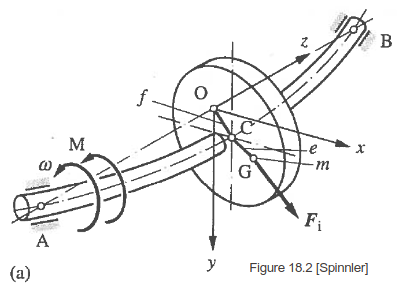
\includegraphics[width=.5\textwidth]{IMAGES/constru/dsm2.png}
\end{figure}

L'équation du mouvement est donnée par : $-k_R y - c_R \dot{y} - m \Ddot{y}_G - mg = 0$\\
On a donc un oscillateur forcé en x et y. Le mouvement du centre du disque C est donné par $x = X \sin(\omega t - \varphi)$, $y = Y \cos(\omega t - \varphi) + \frac{mg}{k}$, $X = Y = e \mu_3$, $\mu_3 = \frac{\beta^2}{\sqrt{(1-\beta^2)^2 + 4\eta^2 \beta^2}}$, $\varphi = \arctan(\frac{2\eta \beta}{1-\beta^2})$.\\
Pour $\beta>>1$, on a une asymptote de $\mu_3$ en 1.\\
\begin{itemize}
    \item Régime sous-critique $\beta<1$ : $\varphi < 90^\circ$, $\Vec{O'G} = \frac{1}{1-\beta^2} e$\\
    \item Régime critique $\beta = 1$ : $\varphi = 90^\circ$, $\Vec{O'G} = \sqrt{1+4\eta^2} \frac{e}{2\eta}$\\
    \item Régime sur-critique $\beta>1$ : $\varphi \simeq 180^\circ$, $\Vec{O'G} \simeq 0$\\
\end{itemize}

Chaque rotor a une vitesse critique. Le rotor de Jeffcott assume des paliers infiniment rigides. La rigidité globale du système vaut : $k = \frac{k_S k_R}{ k_S + k_R}$. On a une amplitude maximale pour $\beta = \frac{1}{\sqrt{1-2\eta^2}}$\\
La rigidité des paliers a un effet significatif sur la forme des modes propres. Pour des arbres souples sur paliers rigides, la déformation de l'arbre domine les modes propres. Pour des arbres rigides sur paliers souples, les modes propres sollicitent les paliers.\\

On obtient un système à 4 DOF : $M\Ddot{\Vec{q}} + G\dot{\Vec{q}} + K\Vec{q} = \Vec{f}$.\\

Les balourds induisent des forces forward (qui tournent avec le rotor). L'évolution des fréquences propres avec la vitesse de rotation se fait grâce au diagramme de Campbell.\\


\end{document}